%!TEX root = ../pres.tex

\begin{frame}
	\frametitle{Behavioral Cloning}
	\begin{center}
		\textbf{Behavioral Cloning:} Supervised learning in MDPs using and expert agent expert $\pi^*$!
	\end{center}
	Given expert examples $\scriptd = (s_t, a_t = \pi^*(s_t))$ and a model $\pi_\theta$ find $\theta^*$ st
	\begin{equation*}
		\theta^*  = \argmin_\theta \scriptl(a_t, \pi_\theta(s_t)).
	\end{equation*}
	where $\scriptl$ is some loss function.
	\begin{itemize}
		\item  Show, don't tell! 
		\item No complicated machinery, just standard ML.
	\end{itemize}
\end{frame}


\begin{frame}
	\frametitle{Behavioral Cloning}
		\textbf{Issue: Compounding Error}
		\begin{columns}
			\begin{column}{0.5\textwidth}
			Given some irreducible error $\epsilon =0.001$
				\begin{itemize}
					\item $\scriptl(a_0, \pi(s_0)) = \epsilon$
					\item $\scriptl(a_1, \pi(s_1)) = 2\epsilon$
					\item $\scriptl(a_2, \pi(s_2)) = 3\epsilon$
					\item $\scriptl(a_3, \pi(s_3)) = 4\epsilon$
					\item $\scriptl(a_4, \pi(s_4)) = 5\epsilon$
				\end{itemize}
			\end{column}
			\begin{column}{0.5\textwidth}
				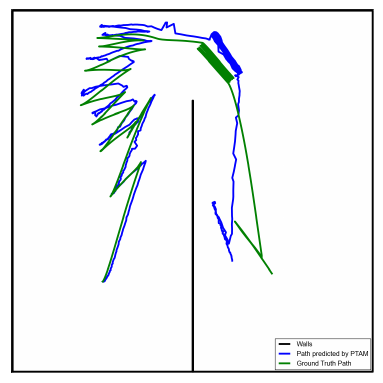
\includegraphics[width=0.99\textwidth]{bh1.png}
			\end{column}
		\end{columns}
\end{frame}